To verify the correctness of the VHDL design files, we have written a C++ program that generates test cases. This program first generates test input with random noise. Then it computes the output using the equivalent filter algorithm in Q15 format. The result is stored in a text file (Appendix \ref{lst:testcase.txt}) which can be read by a VHDL testbench \texttt{filter\_tb.vhd} (Appendix \ref{lst:filter_tb.vhd}).

\begin{figure}[ht]
	\centering
	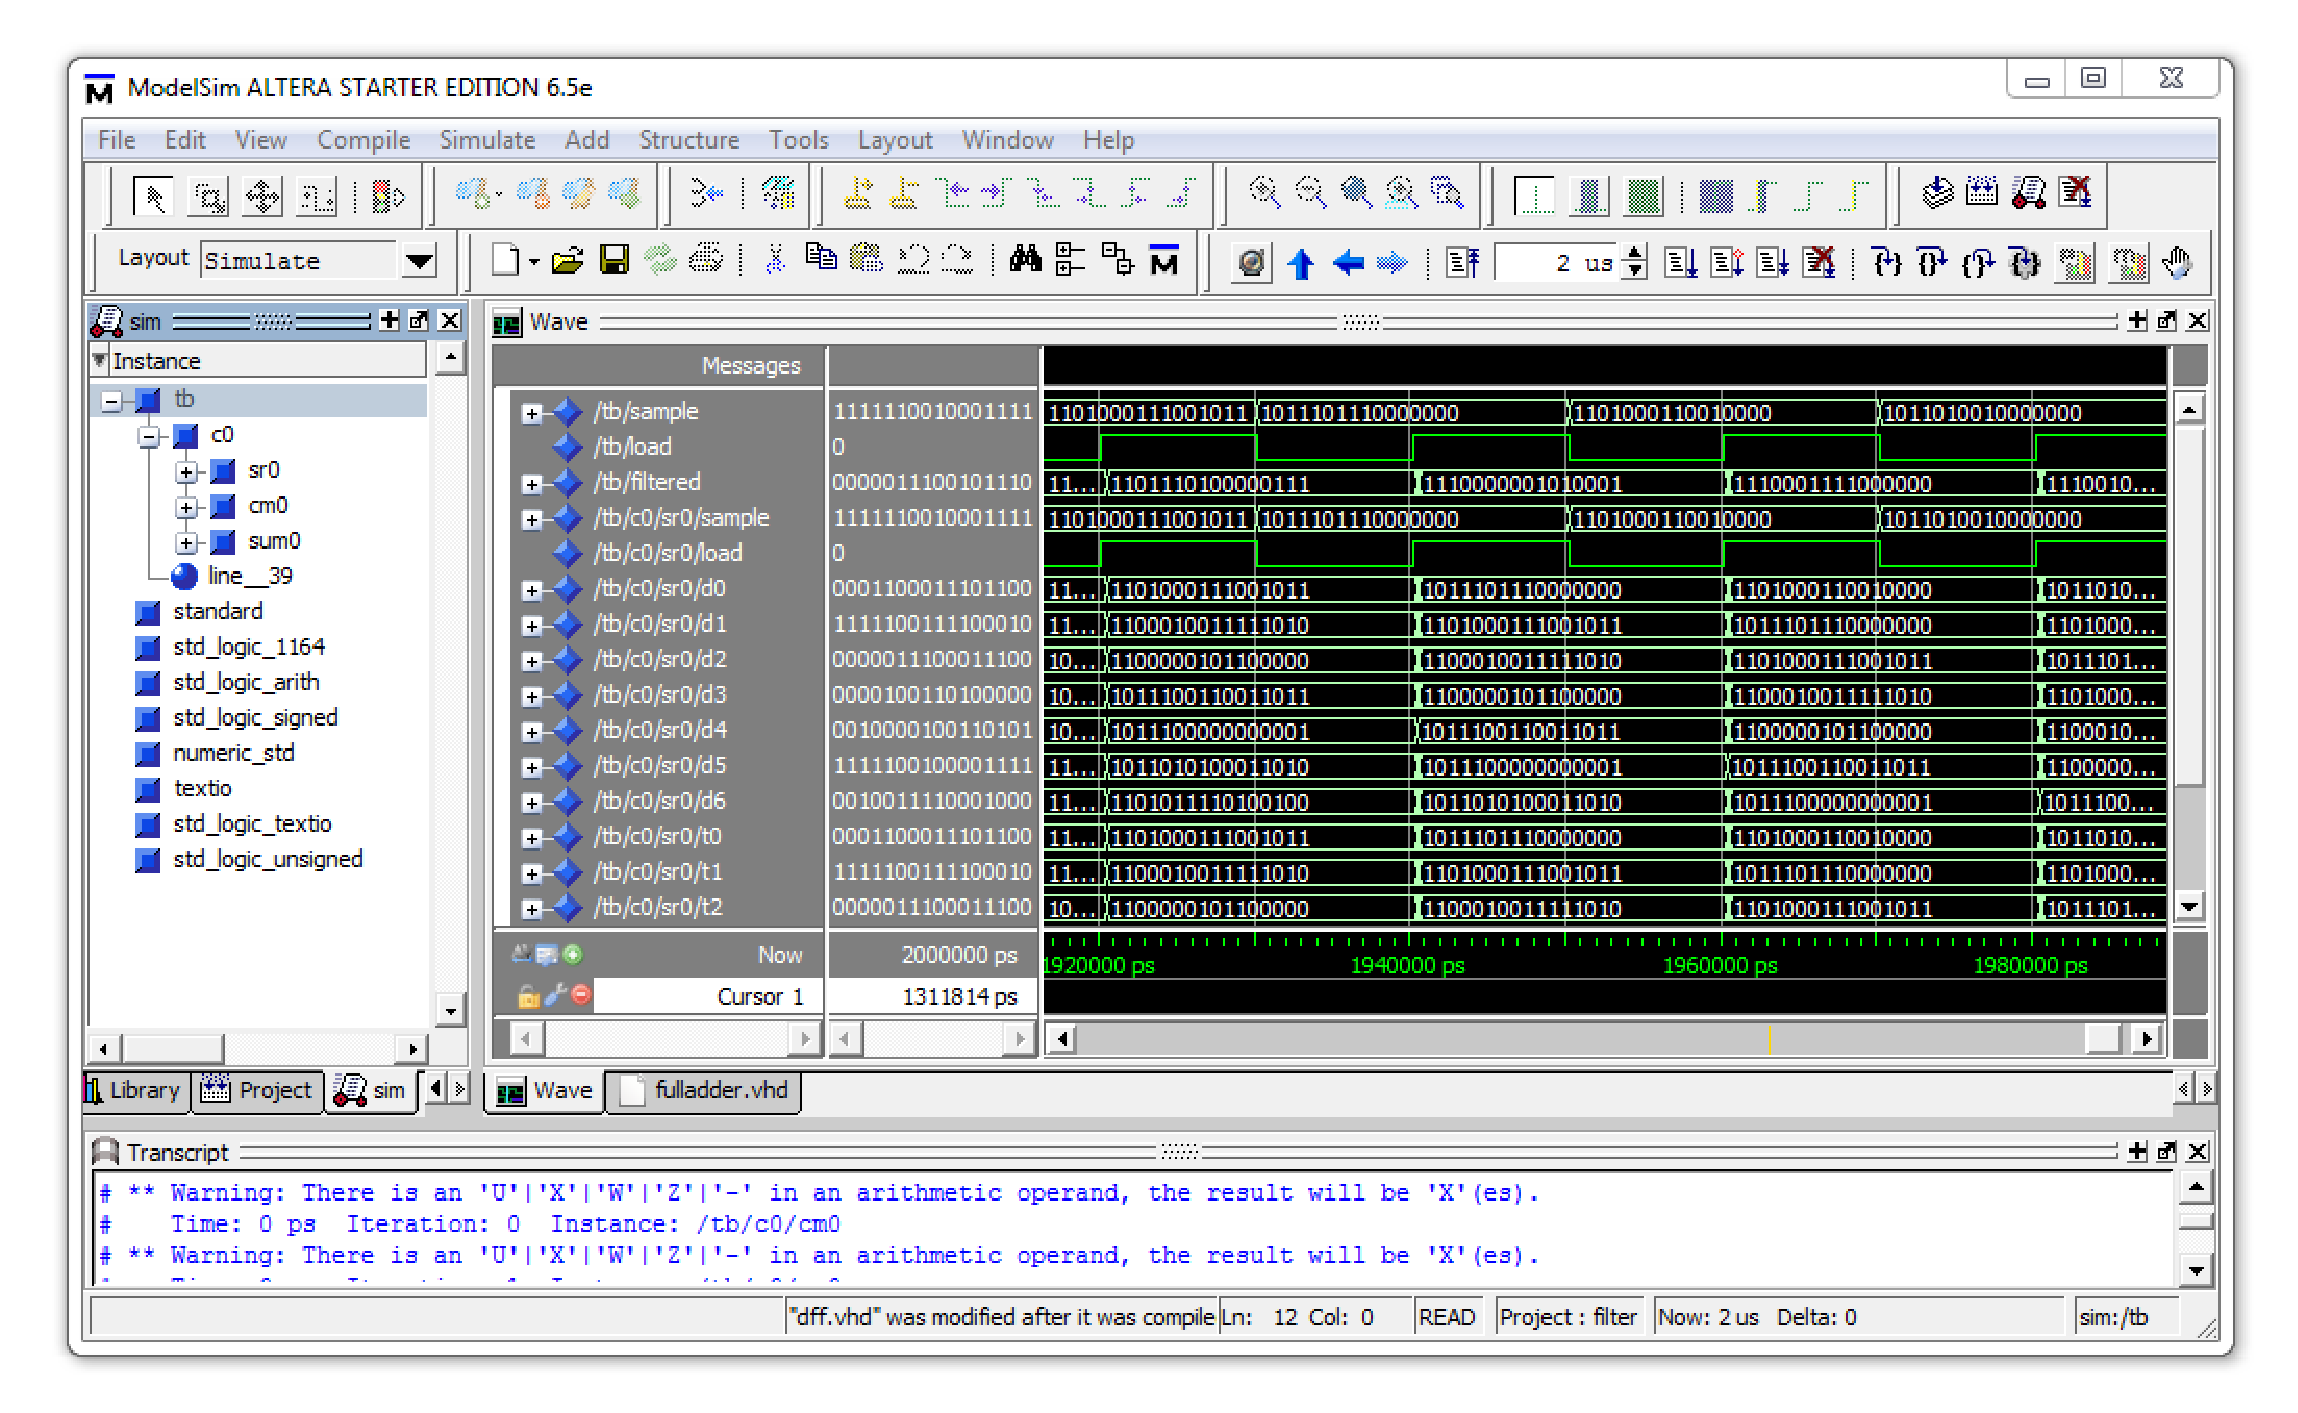
\includegraphics[width=6.5in]{images/modelsim}
	\caption{ModelSim from Mentor Graphics was used for VHDL simulation.}
	\label{fig:q7}
\end{figure}

For VHDL simulation, we used ModelSim from Mentor Graphics. This tools loads and compiles all VHDL files including the test bench, then shows the waveform and output to the window. Our testbench file follows the VHDL standard and prints the results into a text file, so it should work on other environments other than ModelSim.

We verified that the every bit of the C++ program output and VHDL testbench output matched, therefore the VHDL should be correct with high probability.